\documentclass[11pt,a4paper]{article}

\usepackage[margin=2.4cm]{geometry}
\usepackage{booktabs}
\usepackage{graphicx}
\usepackage{amsmath,amssymb}
\usepackage{xcolor}
\usepackage{longtable}
\usepackage{enumitem}
\usepackage{caption}
\usepackage[colorlinks=true,linkcolor=black,urlcolor=blue,citecolor=black]{hyperref}
\usepackage{titlesec}
\usepackage{fancyhdr}

\definecolor{ok}{HTML}{1BAF7A}
\definecolor{open}{HTML}{EB6834}
\definecolor{soft}{HTML}{52514E}
\definecolor{rule}{HTML}{E6E5E1}

\newcommand{\closed}{\textcolor{ok}{\textbf{CLOSED}}}
\newcommand{\opn}{\textcolor{open}{\textbf{OPEN}}}
\newcommand{\refuted}{\textcolor{soft}{\textbf{REFUTED}}}
\newcommand{\evar}{\mathrm{EVaR}}
\newcommand{\cvar}{\mathrm{CVaR}}

\titleformat{\section}{\Large\bfseries}{\thesection}{0.6em}{}
\titleformat{\subsection}{\large\bfseries}{\thesubsection}{0.6em}{}

\pagestyle{fancy}
\fancyhf{}
\lhead{\small\textcolor{soft}{EVaR in distributional deep RL --- status report}}
\rhead{\small\textcolor{soft}{\thepage}}
\renewcommand{\headrulewidth}{0.4pt}

\captionsetup{font=small,labelfont=bf}

\title{\vspace{-1.5cm}\textbf{Risk-Seeking EVaR in Distributional Deep RL}\\[0.3em]
\large Porting multi-timescale SPSA EVaR optimisation to a distributional
actor--critic:\\ method, implementation, measurements, and the state of the evidence}
\author{Status report for collaborators}
\date{}

\begin{document}
\maketitle
\thispagestyle{fancy}
\vspace{-1.2cm}

\begin{center}
\begin{minipage}{0.93\textwidth}
\small\textcolor{soft}{
This report documents a port of the TMLR method \emph{Risk-Seeking Reinforcement
Learning via Multi-Timescale EVaR Optimization} (SPSA-based) into a distributional
deep RL setting, and states precisely what has been established, what has been
refuted, and what remains open. It is deliberately explicit about negative and
null results: several plausible hypotheses were tested and failed, and two
implementation faults produced numbers that looked like findings before they were
caught. Both are documented here, because the diagnostics that caught them are now
part of the method.}
\end{minipage}
\end{center}

\vspace{0.6em}
\hrule
\vspace{0.9em}

\section{Executive summary}

The work has three claims to defend, inherited from the source paper. Their status:

\begin{center}
\small
\begin{tabular}{@{}p{0.055\textwidth}p{0.40\textwidth}p{0.12\textwidth}p{0.36\textwidth}@{}}
\toprule
\textbf{ID} & \textbf{Claim} & \textbf{Status} & \textbf{Evidence} \\
\midrule
C1 & The method optimises the intended objective:
     $\evar_\alpha$ of trajectory returns rises, $\alpha$ moves the tail
     monotonically, $\alpha=1$ recovers risk-neutral
   & \closed{} \newline (exactly) &
     Exact regret $0.00\%$ at all seven $\alpha$ on the lottery gridworld with a
     perfect critic; $\alpha=1$ control exact \\[0.4em]
C2 & It is cheaper than SPSA at matched sample budget
   & \textcolor{soft}{\textbf{ARGUED}} &
     Settled analytically by decision, not by a head-to-head: SPSA spends $2N_t$
     rollouts per update to estimate a scalar, this spends one backprop. The
     paper's published numbers stand for the SPSA side \\[0.4em]
C3 & The per-state approximation is sound
   & \closed{} \newline (reformulated) &
     Was not an approximation gap but a \emph{formulation error}. State-value form
     costs up to $86.35\%$; action-value form is exact ($0.00\%$) \\
\bottomrule
\end{tabular}
\end{center}

\vspace{0.5em}
\noindent\textbf{The one-line state of play.} The operator is correct and now has a
learner capable of standard continuous-control benchmarks. What is \emph{not} yet
established is that EVaR outperforms the standard distortion risk measures; on
every environment tested so far the arms tie, and in each case we can now say
\emph{why} they tie, which is a precondition for fixing it rather than a result.

\vspace{0.5em}
\noindent\textbf{What changed most recently.} A latent fault made the EVaR estimate
scale-dependent: the dual variable $x^\ast = 1/\beta^\ast$ carries units of return,
so a fixed search interval silently degenerated EVaR into fixed-$\beta$ entropic
utility on any environment whose returns are small. Measured error reached
$1100\%$. This is fixed, instrumented, and --- because the fix is essentially
``adapt $\beta$ to the distribution'' --- is the most promising seed for the
intended contribution.

\section{Background: what is being ported}

\subsection{The source method}

The source paper optimises
\begin{equation}
J_{\evar}(\theta) \;=\; \evar_\alpha\big[R(\tau)\big], \qquad \tau \sim \pi_\theta,
\end{equation}
with a two-timescale stochastic-approximation recursion. Because no gradient of
$J_{\evar}$ is available, the policy is perturbed with SPSA, requiring $2N_t$
rollouts per policy update purely to estimate a scalar.

\subsection{Entropic Value-at-Risk}

For a return $Z$ and confidence $\alpha \in (0,1]$,
\begin{equation}
\evar_\alpha[Z] \;=\; \min_{\beta > 0}\; \frac{1}{\beta}
\Big(\log \mathbb{E}\big[e^{\beta Z}\big] - \log \alpha\Big).
\label{eq:evar}
\end{equation}
Under the reparameterisation $x = 1/\beta$ this becomes minimisation of
\begin{equation}
G(x) \;=\; x\Big(\log \mathbb{E}\big[e^{Z/x}\big] - \log\alpha\Big),
\label{eq:G}
\end{equation}
which is strongly convex on a compact interval, so $G'$ is monotone and a sign
change brackets the minimiser. Two properties drive nearly every design decision
that follows:

\begin{enumerate}[leftmargin=1.4em,itemsep=0.25em]
\item \textbf{Translation equivariance.} $\evar_\alpha[c + Z] = c + \evar_\alpha[Z]$
      for scalar $c$. A constant passes through the tilt untouched.
\item \textbf{$x^\ast$ has units of return.} $G$ is homogeneous of degree one:
      rescaling $Z$ by $\lambda$ rescales both $\evar$ and $x^\ast$ by $\lambda$.
      Empirically $x^\ast \approx 0.34\,\mathrm{sd}(Z)$ for Gaussian returns
      (Fig.~\ref{fig:scale}).
\end{enumerate}

\subsection{What the port replaces}

A distributional critic supplies an explicit, differentiable return distribution,
so \eqref{eq:G} can be minimised directly per state and differentiated, replacing
the outer SPSA loop. One backpropagation replaces $2N_t$ rollouts. The remainder of
this report is about what that substitution requires to be correct.

\section{Method}

\subsection{The formulation error: why the critic must be an action-value}

This is the single most consequential finding and it was originally misdiagnosed as
an approximation gap.

The natural per-state advantage is
$A(s,a) = r + \evar_\alpha(Z(s'))$. This is \emph{risk-neutral in the reward}. By
translation equivariance, a \emph{sampled scalar} reward $r$ inside the tilt is
identical to $r$ outside it, so $\evar_\alpha(r + Z(s')) \equiv r +
\evar_\alpha(Z(s'))$. At a terminal step $Z(s')$ is degenerate, $\alpha$ cannot
enter at all, and the comparison reduces to safe-reward against lottery
\emph{mean}. That makes the previous step deterministic, and the collapse
propagates backwards: the fixed point is the risk-neutral policy at every $\alpha$.

The tilt reaches the reward only when the critic represents the reward's
\emph{distribution}, i.e.\ $Z(s,a)$. Measured exactly on the lottery gridworld with
a perfect critic and greedy improvement (no learning, so the numbers are exact):

\begin{center}
\small
\begin{tabular}{@{}lcc@{}}
\toprule
\textbf{Advantage form} & \textbf{$\alpha$ values correct} & \textbf{Worst exact regret} \\
\midrule
$r + \evar_\alpha(Z(s'))$ \quad (state-value) & 1 of 7 & $86.35\%$ \\
$\evar_\alpha(Z(s,a))$ \quad (action-value) & \textbf{7 of 7} & $\mathbf{0.00\%}$ \\
\bottomrule
\end{tabular}
\end{center}

\noindent The mechanism is visible in the solved duals: the trajectory objective
decouples at one \emph{global} $x^\ast$, while the per-state solve uses a different
$x^\ast(s)$ at each state. At $\alpha = 0.10$, global $x^\ast = 36.54$ while the
per-state solve gives $36.54$, $36.54$, $0.00$ at the three decision columns --- the
terminal column collapses to zero, which is precisely the degeneracy above.

\subsection{The distributional critic}

$Z(s,a)$ is represented by implicit quantiles (IQN) rather than a fixed categorical
support. The reason is concrete rather than aesthetic: C51 requires $v_{\min},
v_{\max}$ in the units the critic actually represents --- \emph{discounted} return,
not undiscounted episode return. Getting this wrong left $\approx 9$ of $51$ atoms
carrying any mass on CartPole and $\approx 5$ of $51$ on InvertedPendulum, and
since EVaR is a tail statistic read off exactly that histogram, the operator was
being fed a 9-point support. Quantiles have no support to mis-size and place
resolution where the distribution is.

The critic embeds state--action and quantile level separately and combines them
multiplicatively:
\begin{equation}
Z_\tau(s,a) = f\Big(\psi(s,a) \odot \phi(\tau)\Big), \qquad
\phi_j(\tau) = \mathrm{ReLU}\Big(\textstyle\sum_{i} \cos(\pi i \tau)\,w_{ij} + b_j\Big),
\end{equation}
trained with the quantile Huber loss over all $(\tau_i, \text{target}_j)$ pairs.

\subsection{The inner solve}

\textbf{Bisection, not Newton.} The original projected-Newton solve never
converged. When the tilted measure collapses onto one atom, $\mathrm{Var}_{Q_x}
\to 0$, the curvature $G'' = \mathrm{Var}_{Q_x}/x^3$ underflows its clamp, the step
$G'/G''$ explodes, is projected onto a bound, and cycles between the bounds
forever. The returned $x^\ast$ was whichever bound the step-count parity landed on
--- constant at $0.301$ across genuinely different return distributions --- and EVaR
was inflated by $25$--$590\%$, with the error \emph{growing in the scale of
returns}, i.e.\ in the same direction as C1 itself. Bisecting the monotone $G'$ in
$\log x$ converges unconditionally and now matches brute-force minimisation to
$0.00\%$.

\textbf{Gradients by the envelope theorem.} $x^\ast$ is detached. Since
$\partial G/\partial x = 0$ at the optimum, $\mathrm{d}G/\mathrm{d}\theta =
\partial G/\partial\theta$ evaluated at $x^\ast$, so gradients into the critic are
exact without unrolling the solver --- and, unlike an unrolled loop, cannot be
corrupted by the iteration's own conditioning. Checked against finite differences at
$5\times 10^{-9}$.

\textbf{Zero-probability atoms are masked, not floored.} A \texttt{clamp\_min(1e-12)}
does not guard $\log 0$ harmlessly: it \emph{invents} mass $10^{-12}$ on atoms whose
true probability is zero, and the tilt $e^{Z/x}$ multiplies that fake mass by
$e^{z_{\max}/x}$. On a C51 support up to $500$ with $x \approx 11$ that is a factor
of $e^{45}$, enough for a floored atom to dominate $Q_x$ and pull EVaR up by
$13.3\%$. Genuine zeros are masked to $-\infty$ instead.

\textbf{The saturated regime is returned exactly.} $G'(0^+) = \log(p_{\max}/\alpha)$
where $p_{\max}$ is the mass on the largest atom, so once $p_{\max} \ge \alpha$ the
objective is non-decreasing everywhere and the infimum sits at $x \to 0$, where
$G \to z_{\max}$. EVaR then \emph{is} the maximum. Bisecting anyway lands on
$x_{\min}$ and returns $z_{\max} + x_{\min}\log(1/\alpha)$, breaking the invariant
$\mathbb{E}[Z] \le \evar_\alpha[Z] \le \max(Z)$.

\subsection{Scale-adaptive dual interval (new)}

Because $x^\ast$ has units of return, a fixed interval $[x_{\min}, x_{\max}]$ is
only valid at one return scale. Figure~\ref{fig:scale} shows the consequence.

\begin{figure}[h]
\centering
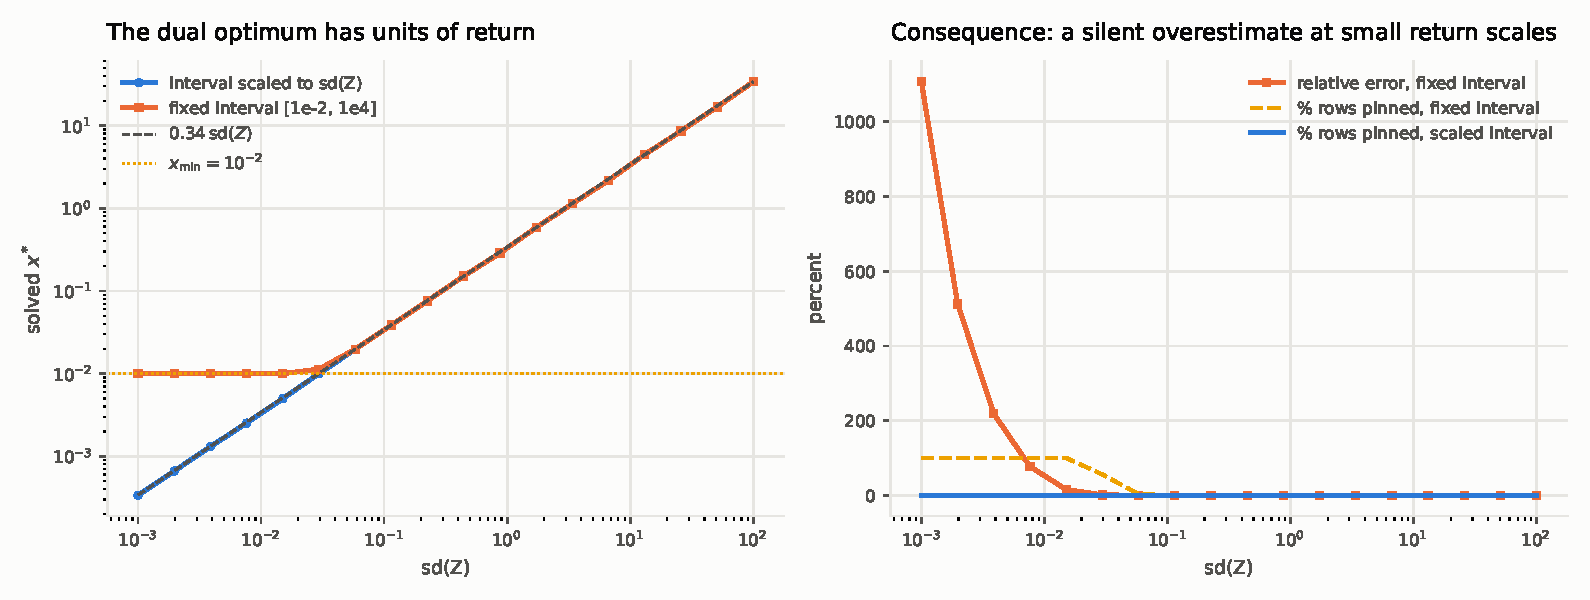
\includegraphics[width=\textwidth]{figures/solver_scale.pdf}
\caption{\textbf{Left:} the solved dual $x^\ast$ tracks $0.34\,\mathrm{sd}(Z)$ over
five orders of magnitude. With a fixed interval it flattens onto $x_{\min}=10^{-2}$
as soon as the true optimum falls below it. \textbf{Right:} the resulting relative
error in EVaR, reaching $1100\%$ at $\mathrm{sd}(Z)=10^{-3}$, alongside the fraction
of rows pinned at a bound. With the interval derived per row from $\mathrm{sd}(Z)$,
nothing pins at any scale.}
\label{fig:scale}
\end{figure}

At the bound, EVaR equals $\text{mean} + x_{\min}\log(1/\alpha)$ exactly --- that is
fixed-$\beta$ entropic utility, which is precisely the baseline the dual solve
exists to beat. The interval is now derived per row as
$[10^{-3}\,\mathrm{sd}(Z),\; 10^{3}\,\mathrm{sd}(Z)]$, with the absolute bounds
retained as fallbacks for degenerate rows. Validated against brute-force
minimisation over a dense logarithmic grid: maximum relative error $5\times10^{-6}$
from $\mathrm{sd}(Z)=100$ down to $\mathrm{sd}(Z)=0.001$.

\emph{Why this matters beyond being a bugfix.} It is a measured demonstration that
the tilt strength must adapt to the distribution it is applied to. That is the same
argument as adaptive $\beta$, with a failure mode behind it instead of an
intuition.

\begin{figure}[h]
\centering
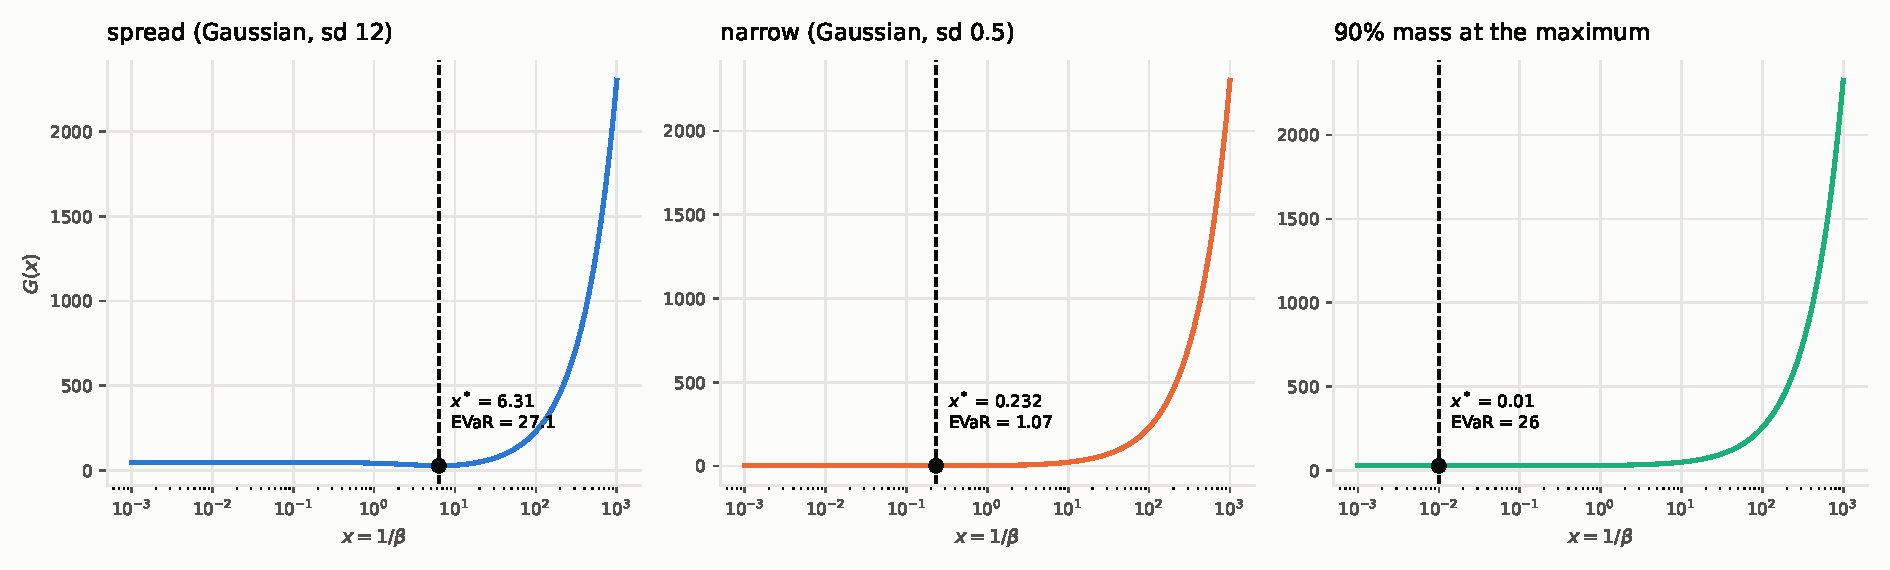
\includegraphics[width=\textwidth]{figures/dual_objective.pdf}
\caption{The dual objective $G(x)$ for three distribution shapes with the solved
optimum marked. Left and centre: an interior minimum, correctly located at very
different $x$ for the same $\alpha$. Right: with $90\%$ of the mass at the maximum
the optimum is driven toward $x \to 0$ and EVaR approaches $\max(Z)$ --- the
saturated regime, which is detected and returned exactly rather than bisected.}
\label{fig:dual}
\end{figure}

\subsection{Solver budget}

\begin{figure}[h]
\centering
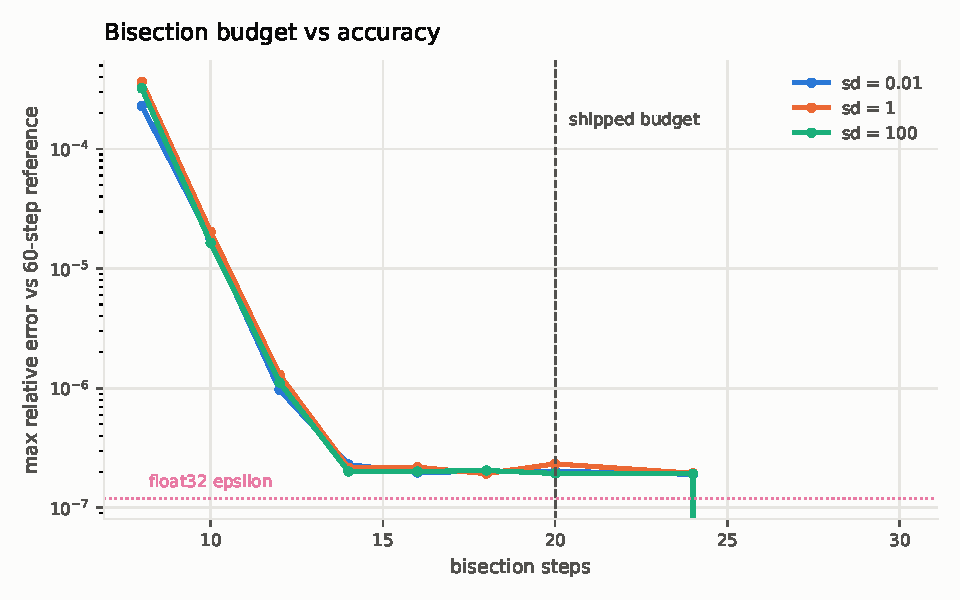
\includegraphics[width=0.66\textwidth]{figures/solver_precision.pdf}
\caption{Accuracy against a 60-step reference. The shipped budget of 20 bisections
sits at float32 machine epsilon across return scales; 30 bought nothing measurable
while costing $\approx 12$ kernel launches each.}
\label{fig:precision}
\end{figure}

\section{The learner}

\subsection{Rationale}

Two earlier learners failed for recorded reasons. The $n$-step A2C could not do
continuous control at all --- on \texttt{SafetyPointGoal1} with cost priced at zero
it sat at random-policy reward for 1500 episodes. The on-policy PPO learner works
but is sample-hungry, and this literature runs continuous control off-policy. The
current learner is a risk-sensitive DSAC.

\begin{description}[leftmargin=1.2em,itemsep=0.25em]
\item[Off-policy with replay.] The comparisons that matter on continuous control
  are off-policy; it also means the tail is estimated from the whole buffer rather
  than one rollout, which is the regime the risk measure needs.
\item[IQN action-value critic.] $\evar(Z(s,a))$, never $r + \evar(Z(s'))$, for the
  reason in \S3.1.
\item[Twin critics, minimum over the \emph{risk} value.] Standard overestimation
  control, applied to the quantity the actor actually maximises.
\item[Tanh-squashed actor.] A clamped Gaussian returns the density of the
  \emph{unclamped} sample, so any objective comparing densities of executed actions
  evaluates them at a boundary where the density swings violently once the mean
  drifts outside the bound. In the PPO learner this produced approximate KL of
  $64$ and then $1.4\times10^{16}$, killing runs outright. Tanh squashing has no
  boundary; the log-probability carries the exact Jacobian correction
  $\log(1-\tanh^2 u) = 2(\log 2 - u - \mathrm{softplus}(-2u))$.
\item[Automatic entropy temperature.] Hand-tuning wasted real time earlier: at
  $10^{-3}$ and $10^{-2}$ policy entropy collapsed identically, because the
  coefficient is scaled against \emph{normalised} advantages. The fix was removing
  the constant, not choosing a better one.
\item[Pluggable risk functional.] \texttt{--risk mean} is a true risk-neutral
  control sharing critic, actor, data and seeds. It is the only thing that licenses
  attributing a difference to the risk measure.
\end{description}

\subsection{Update}

Per environment step, one gradient update. Critic target (with $d$ the
\emph{termination} flag only, so time-limit truncation still bootstraps):
\begin{equation}
y_j = r - \lambda c \;+\; \gamma (1-d)\Big(\min_{k\in\{1,2\}} Z^{\text{targ}}_{k,\tau_j}(s',a')
      \;-\; \eta \log \pi(a'|s')\Big), \qquad a' \sim \pi(\cdot|s'),
\end{equation}
regressed with the quantile Huber loss. Actor objective, maximising the risk value
rather than the mean:
\begin{equation}
\mathcal{L}_\pi = \mathbb{E}_s\Big[\eta \log\pi(a|s) \;-\;
  \min_{k\in\{1,2\}} \rho_\alpha\big(Z_k(s,a)\big)\Big], \qquad a \sim \pi(\cdot|s),
\end{equation}
with $\rho_\alpha$ the selected risk functional ($\evar_\alpha$, mean, $\cvar$,
Wang, CPW, fixed-$\beta$ entropic, or mean--variance).

\subsection{Constraint: $\alpha > 1/K$}

On a $K$-sample empirical measure the top sample carries mass $1/K$. Once that
reaches $\alpha$ the dual optimum runs to $x_{\min}$ and EVaR collapses onto the
sample maximum. With $K = 64$ risk quantiles the floor is $\alpha > 0.0156$. This
is checked at construction and raises rather than silently saturating. The same
constraint binds independently on evaluation sample size; an early $\alpha = 0.01$
sweep was invalid in all 500 of its evaluation rows for this reason.

\section{Hyperparameters and implementation}

\begin{center}
\small
\begin{longtable}{@{}p{0.34\textwidth}p{0.21\textwidth}p{0.41\textwidth}@{}}
\toprule
\textbf{Parameter} & \textbf{Value} & \textbf{Note} \\
\midrule
\endhead
\multicolumn{3}{@{}l}{\textit{Risk operator} (\texttt{evar\_deeprl/risk/evar.py})}\\
\midrule
$\alpha$ & $0.1$ & risk level; $\alpha=1$ is the exact risk-neutral control \\
\texttt{solver\_steps} & $20$ & bisections; float32 epsilon (Fig.~\ref{fig:precision}) \\
\texttt{auto\_scale\_bounds} & \texttt{True} & per-row interval from $\mathrm{sd}(Z)$ \\
\texttt{rel\_x\_min}, \texttt{rel\_x\_max} & $10^{-3}$, $10^{3}$ & multiples of $\mathrm{sd}(Z)$ \\
\texttt{x\_min}, \texttt{x\_max} & $10^{-2}$, $10^{4}$ & absolute fallback for degenerate rows \\
gradient path & envelope theorem & $x^\ast$ detached; FD-checked at $5\times10^{-9}$ \\
\midrule
\multicolumn{3}{@{}l}{\textit{IQN action-value critic} (\texttt{distributional/iqn\_q.py})}\\
\midrule
hidden sizes & $(256, 256)$ & state--action encoder, ReLU \\
embedding dim & $128$ & \\
$n_{\cos}$ & $64$ & cosine basis for $\tau$ \\
Huber $\kappa$ & $1.0$ & \\
$K$ critic / target / risk & $32$ / $32$ / $64$ & risk uses more samples; $\alpha > 1/K$ \\
\midrule
\multicolumn{3}{@{}l}{\textit{Actor} (\texttt{policies/squashed\_gaussian.py})}\\
\midrule
hidden sizes & $(256, 256)$ & ReLU \\
$\log\sigma$ clamp & $[-20, 2]$ & \\
squashing & $\tanh$ & exact Jacobian correction \\
\midrule
\multicolumn{3}{@{}l}{\textit{DSAC} (\texttt{agents/dsac\_evar.py})}\\
\midrule
optimiser & Adam & \\
learning rates & $3\times10^{-4}$ & actor, critic, entropy temperature \\
batch size & $256$ & \\
replay capacity & $10^{6}$ & \\
$\gamma$ & $0.99$ & \\
$\tau$ (polyak) & $0.005$ & \\
updates per env step & $1$ & \\
target entropy & $-\dim(\mathcal{A})$ & auto-tuned temperature \\
warm-up (\texttt{start\_steps}) & $2000$--$5000$ & uniform random actions \\
bootstrap flag & \texttt{terminated} only & truncation still bootstraps \\
cost pricing & $r_{\text{eff}} = r - \lambda c$ & $\lambda = 0$ in the runs reported here \\
\bottomrule
\end{longtable}
\end{center}

\section{Diagnostics and invariants}

Every one of these was added because it caught a real fault. They are logged each
update.

\begin{center}
\small
\begin{tabular}{@{}p{0.26\textwidth}p{0.20\textwidth}p{0.48\textwidth}@{}}
\toprule
\textbf{Diagnostic} & \textbf{Healthy value} & \textbf{What it catches} \\
\midrule
\texttt{at\_bound\_frac} & $0$ for $\alpha<1$ &
  Dual solve landing on its interval: EVaR has degenerated into fixed-$\beta$
  entropic utility. Sat at $1.0$ for every update of every run while Newton was
  broken \\[0.3em]
\texttt{top\_mass\_frac} & $\approx 1/K = 0.0156$ &
  Mass within $0.05\,\mathrm{sd}$ of the maximum. High means the critic produced a
  near-degenerate $Z$ and EVaR is reporting its maximum, not a tail average \\[0.3em]
\texttt{z\_sd\_mean} & task-dependent &
  Spread available to the risk measure. If small relative to return scale, all
  risk attitudes tie \emph{by construction} \\[0.3em]
\texttt{saturated\_frac} & $0$ &
  $p_{\max} \ge \alpha$: EVaR \emph{is} $\max(Z)$ and is returned exactly \\[0.3em]
$\mathbb{E}[Z] \le \evar \le \max Z$ & always &
  Bounds invariant; exposed the saturated regime \\
\bottomrule
\end{tabular}
\end{center}

\noindent\textbf{A cautionary note on diagnostics.} The first version of
\texttt{at\_bound\_frac} was itself wrong: bisection drives \texttt{lo} and
\texttt{hi} onto $x^\ast$, so comparing the solution against the post-loop bounds
compares it against itself, and every solve reported as bound-hitting. It was
caught by calibrating on distributions with known answers --- a Gaussian with
$\mathrm{sd}=12$ reported $\texttt{at\_lower}=1.00$ while $x^\ast=4.05$ sat plainly
interior. \emph{Diagnostics require the same validation as the code they watch.}

\section{Experiments and results}

\subsection{Exact testbed: the lottery gridworld}

A three-segment gridworld where each segment offers a safe payoff or a lottery, and
trajectory EVaR is exactly computable by enumeration. It exists because claims about
tail statistics need a setting where the ground truth is known rather than
estimated.

\begin{figure}[h]
\centering
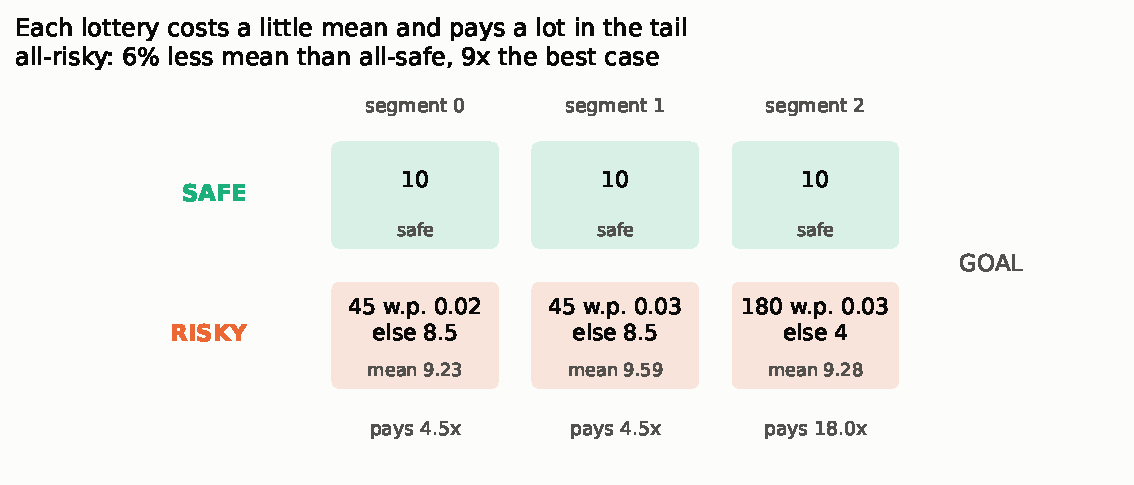
\includegraphics[width=0.86\textwidth]{figures/gridworld_environment.pdf}
\caption{The lottery gridworld. Each risky segment sacrifices a little mean for a
large upper tail: taking all three lotteries gives up $6\%$ of the mean return for
$9\times$ the best case. This asymmetry is deliberate --- a risk-seeking method must
be able to \emph{gain} something by accepting variance, or the benchmark cannot
distinguish it from a broken one.}
\label{fig:gw}
\end{figure}

\begin{figure}[h]
\centering
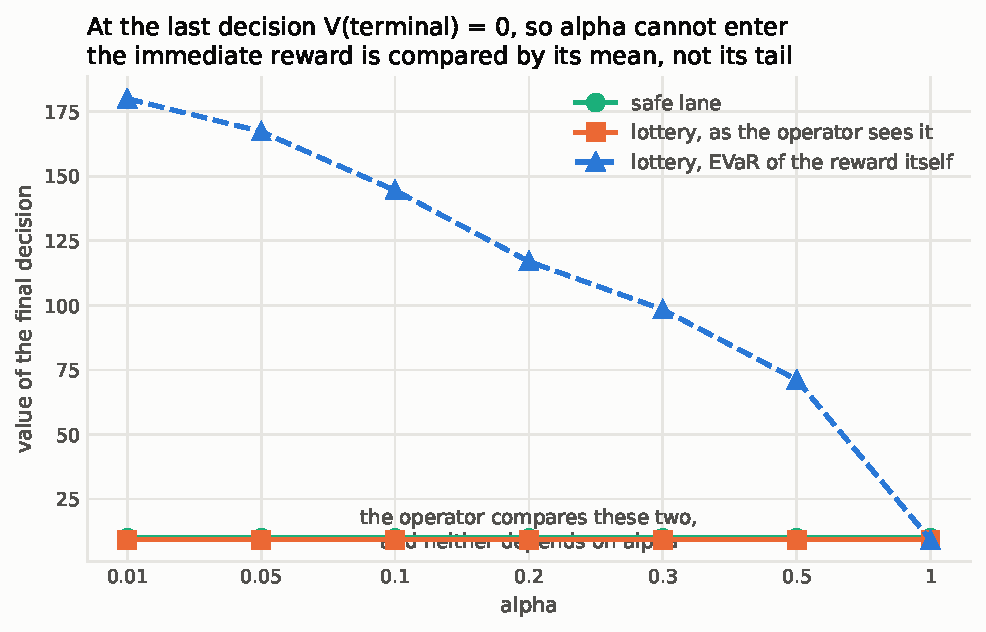
\includegraphics[width=\textwidth]{figures/gridworld_c3_mechanism.pdf}
\caption{The C3 mechanism: how the state-value operator's tilt fails to reach the
sampled reward, and where the per-state dual departs from the global one.}
\label{fig:c3}
\end{figure}

\paragraph{C3, exactly.} With a perfect critic and greedy improvement, so that any
gap is a property of the method and not of an optimiser:

\begin{center}
\small
\begin{tabular}{@{}lllrrr@{}}
\toprule
$\alpha$ & Trajectory optimum & Per-state fixed point & $\evar$ opt & $\evar$ fp & Regret \\
\midrule
0.01 & RISKY-RISKY-RISKY & SAFE-SAFE-SAFE & 219.774 & 30.000 & $86.35\%$ \\
0.05 & SAFE-RISKY-RISKY  & SAFE-SAFE-SAFE & 187.867 & 30.000 & $84.03\%$ \\
0.10 & SAFE-RISKY-RISKY  & SAFE-SAFE-SAFE & 164.835 & 30.000 & $81.80\%$ \\
0.20 & SAFE-RISKY-RISKY  & SAFE-SAFE-SAFE & 137.157 & 30.000 & $78.13\%$ \\
0.30 & SAFE-RISKY-RISKY  & SAFE-SAFE-SAFE & 118.482 & 30.000 & $74.68\%$ \\
0.50 & SAFE-SAFE-RISKY   & SAFE-SAFE-SAFE &  91.223 & 30.000 & $67.11\%$ \\
1.00 & SAFE-SAFE-SAFE    & SAFE-SAFE-SAFE &  30.000 & 30.000 & $0.00\%$ \\
\bottomrule
\end{tabular}
\end{center}

\noindent The state-value form returns the risk-neutral policy at \emph{every}
$\alpha$ --- the signature of the degeneracy in \S3.1. The action-value form
reaches the trajectory optimum at all seven values with $0.00\%$ regret.

\paragraph{Caveat, stated deliberately.} $0.00\%$ is exact \emph{on this
environment}, where segments are independent and the objective decouples. It
establishes that the state-value form is the source of the bias and that the
action-value form removes it here --- not that per-state tilting is exact in
general.

\subsection{Path dependence: a hypothesis tested and refuted}

The literature holds that per-state risk is a proxy for trajectory-level risk and
can be suboptimal. The natural place for that to bite is when segments are
\emph{dependent}, so the decoupling above no longer applies. We broke independence
by making each lottery depend on the lane taken previously:

\begin{center}
\small
\begin{tabular}{@{}lcccc@{}}
\toprule
& \multicolumn{2}{c}{\textbf{Independent segments}} & \multicolumn{2}{c}{\textbf{Path-dependent segments}} \\
\cmidrule(lr){2-3}\cmidrule(lr){4-5}
& state-value & action-value & state-value & action-value \\
\midrule
Worst regret & $86.35\%$ & $\mathbf{0.00\%}$ & $81.29\%$ & $\mathbf{0.00\%}$ \\
\bottomrule
\end{tabular}
\end{center}

\noindent\refuted{} The action-value form stays exact at every $\alpha$ even with
dependence. The premise for a trajectory-consistency contribution does not hold on
this construction, and we should not build on it.

\subsection{Can the risk measures be told apart at all?}

A benchmark is worthless if the methods it compares want the same policy. An
exhaustive search over 28 candidate lottery configurations, scoring six risk
measures by their exact optimal policies, found configurations where \textbf{5 of 6
measures select distinct optima}. Example:

\begin{center}
\small
\begin{tabular}{@{}lll@{}}
\toprule
\textbf{Measure} & \textbf{Optimal policy} & \textbf{Value} \\
\midrule
mean & SAFE-SAFE-SAFE & 30.00 \\
$\evar_{0.1}$ & RISKY-RISKY-SAFE & 83.08 \\
$\cvar_{0.1}$ & RISKY-RISKY-RISKY & 64.19 \\
Wang$_{0.75}$ & SAFE-RISKY-RISKY & 38.14 \\
entropic$_{0.05}$ & SAFE-RISKY-SAFE & 41.56 \\
mean--variance$_{1}$ & SAFE-RISKY-SAFE & 43.15 \\
\bottomrule
\end{tabular}
\end{center}

\noindent This matters for interpreting the null results below: the measures
\emph{are} separable in principle. Where they tie, that is a property of the
environment, not a proof that EVaR is redundant.

\subsection{Pendulum-v1: learner validation}

\begin{figure}[h]
\centering
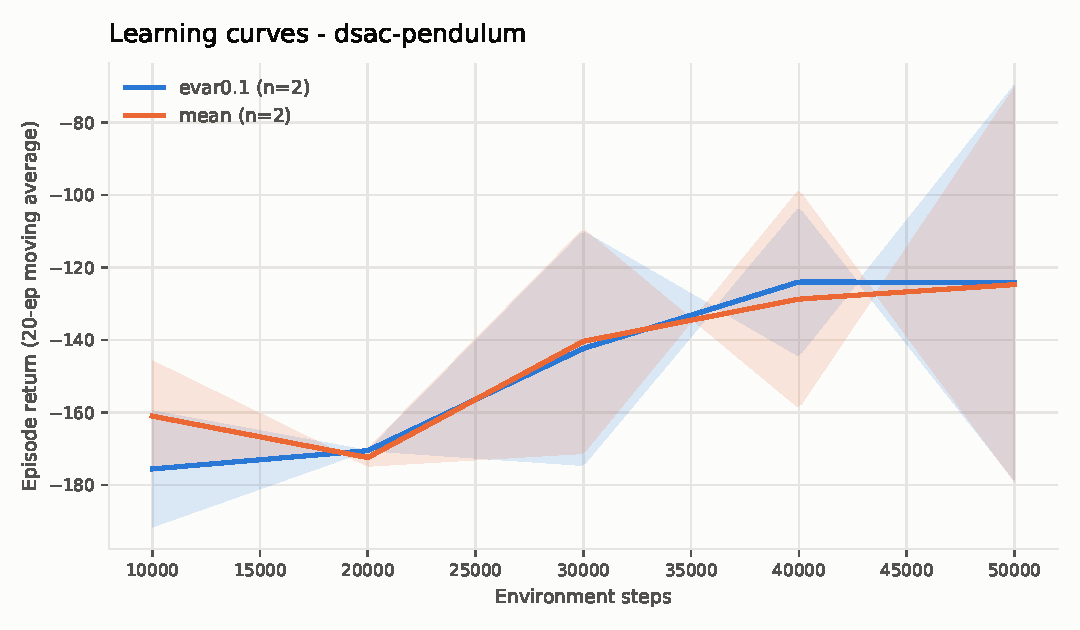
\includegraphics[width=0.49\textwidth]{figures/dsac-pendulum_dsac_return.pdf}
\hfill
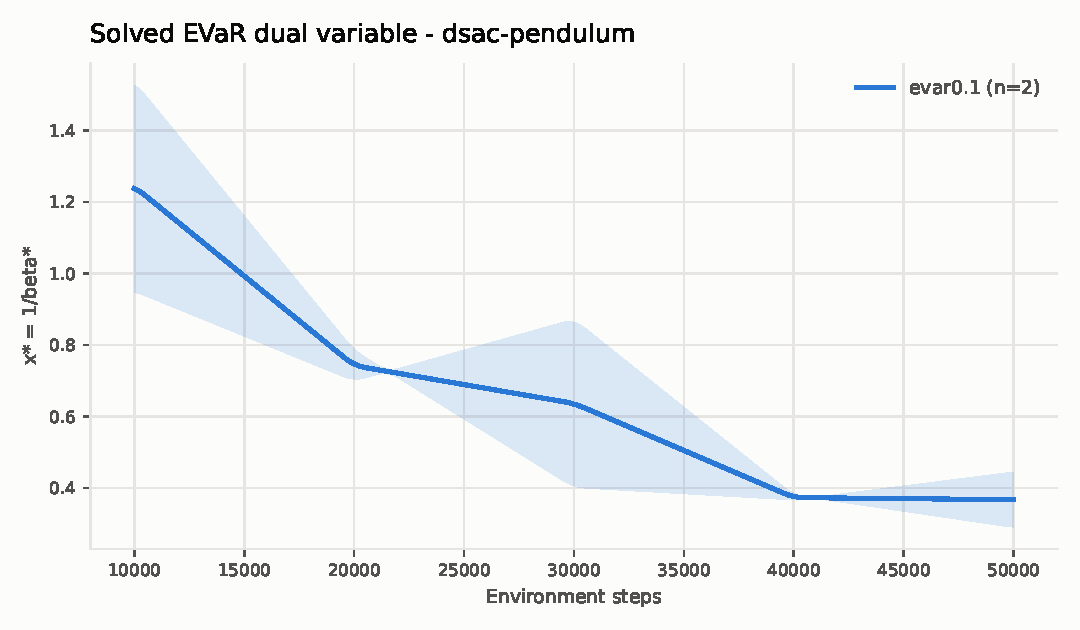
\includegraphics[width=0.49\textwidth]{figures/dsac-pendulum_dsac_dual_x.pdf}
\caption{Pendulum: return (left) and the solved dual $x^\ast$ (right), EVaR arm
against the matched risk-neutral control.}
\label{fig:pend}
\end{figure}

\begin{center}
\small
\begin{tabular}{@{}lrrr@{}}
\toprule
\textbf{Seed} & \textbf{\texttt{mean} control} & \textbf{$\evar_{0.1}$} & \textbf{Paired gap} \\
\midrule
0 & $-96.995$ & $-96.365$ & $+0.63$ \\
1 & $-152.436$ & $-151.919$ & $+0.52$ \\
\bottomrule
\end{tabular}
\end{center}

\noindent Random policy is $\approx -1200$, so both arms solve the task. \textbf{Read
this table by seed, not by arm.} Seed variance is $55$ return points while the
within-seed gap is $0.6$ and $0.5$ --- the arms track each other run for run, which
is much harder to obtain by accident than a matching average.

\textbf{A tie here is the correct outcome, not a null result.} Pendulum's return
spread is policy noise rather than risk in the world, so there is no upper tail to
trade for. This is the same reasoning that retired CartPole, where the risk-neutral
and risk-seeking optima are provably the same policy, the return is capped at 500
and integer-valued (censoring the very tail the operator is defined on), and a
measured sweep produced non-monotone tail statistics with the risk-neutral control
\emph{highest}. What Pendulum validates is plumbing: that the operator is wired in,
that $x^\ast$ solves to an interior value ($0.37$--$0.41$) rather than pinning, and
that switching the functional does not destabilise the learner.

\subsection{SafetyPointGoal1-v0}

\begin{figure}[h]
\centering
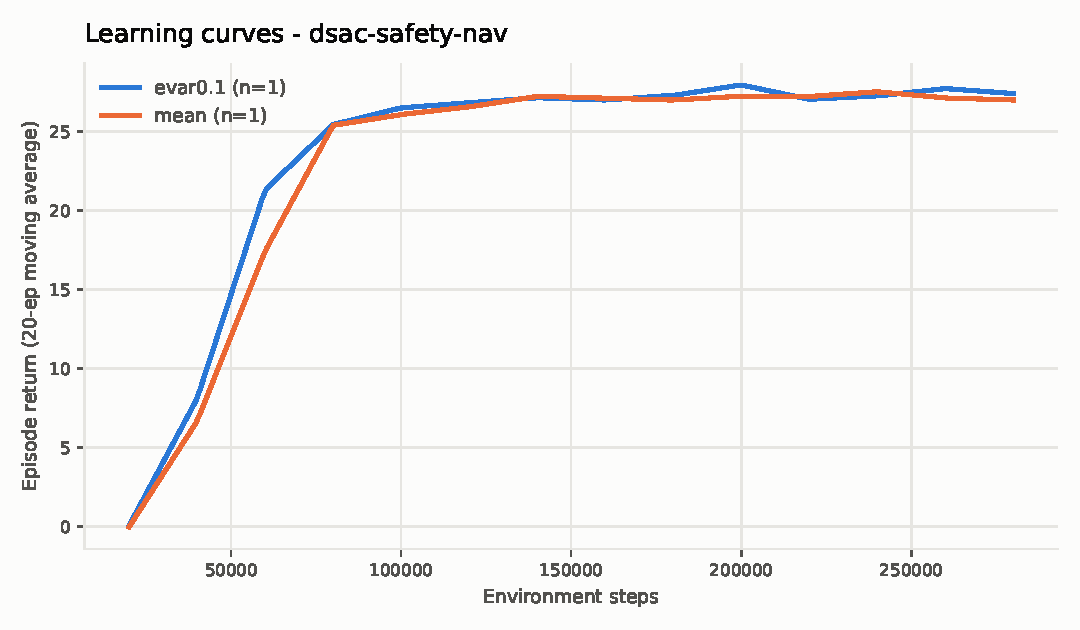
\includegraphics[width=0.49\textwidth]{figures/dsac-safety-nav_dsac_return.pdf}
\hfill
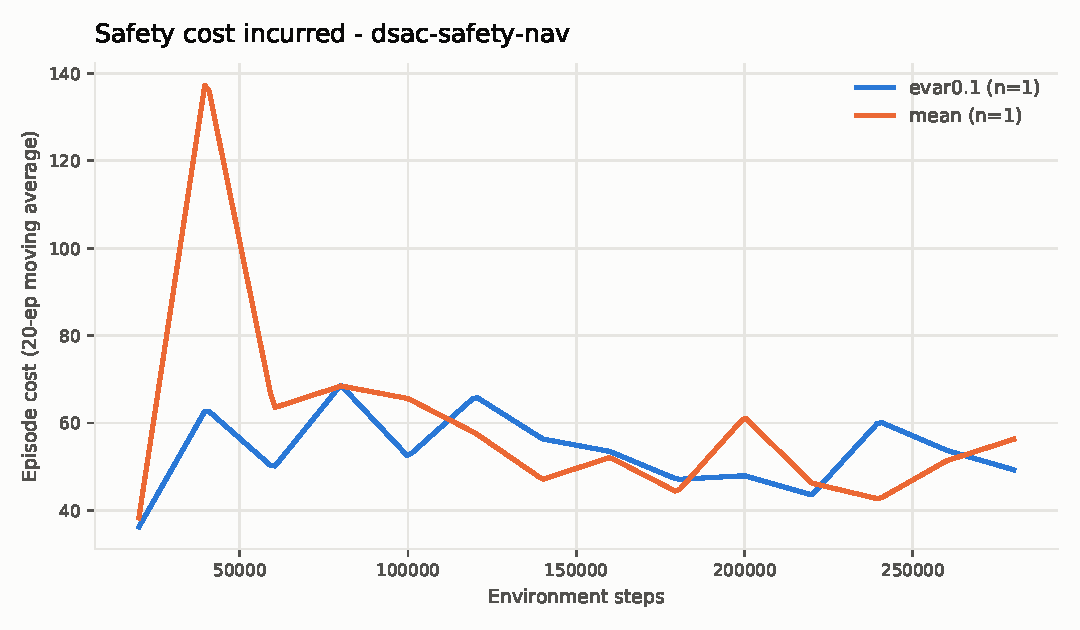
\includegraphics[width=0.49\textwidth]{figures/dsac-safety-nav_dsac_cost.pdf}
\caption{SafetyPointGoal1, 300k steps, cost priced at zero ($\lambda = 0$): return
(left) and incurred safety cost (right).}
\label{fig:safety}
\end{figure}

\begin{center}
\small
\begin{tabular}{@{}lrrr@{}}
\toprule
\textbf{Arm} & \textbf{Final return} & \textbf{Cost} & \textbf{Throughput} \\
\midrule
\texttt{mean} control & $26.986$ & $56.30$ & $62.7$ steps/s \\
$\evar_{0.1}$ & $\mathbf{27.391}$ & $49.30$ & $49.0$ steps/s \\
\bottomrule
\end{tabular}
\end{center}

\noindent\textbf{Result 1: the learner solves the benchmark.} The $n$-step A2C sat
at random-policy reward here for 1500 episodes. This reaches $\approx 27$ and holds.
The continuous-control ladder that blocked everything downstream is open.

\noindent\textbf{Result 2: this environment cannot discriminate risk attitudes},
and that is now measured rather than suspected. A probe run logging the shape of
$Z(s,a)$ throughout training:

\begin{center}
\small
\begin{tabular}{@{}rrrrrr@{}}
\toprule
\textbf{Step} & \textbf{Return} & \textbf{$x^\ast$} & \textbf{$\mathrm{sd}(Z)$} & \textbf{top-mass} & \textbf{at-bound} \\
\midrule
5{,}000  & $-0.00$ & 0.0451 & 0.0754 & 0.017 & $0.00$ \\
10{,}000 & $0.30$  & 0.0168 & 0.0358 & 0.017 & $0.00$ \\
20{,}000 & $0.49$  & 0.0084 & 0.0218 & 0.019 & $0.00$ \\
30{,}000 & $5.73$  & 0.0173 & 0.0240 & 0.017 & $0.00$ \\
35{,}000 & $10.80$ & 0.0122 & 0.0228 & 0.017 & $0.00$ \\
\bottomrule
\end{tabular}
\end{center}

Read in three parts. \texttt{at-bound} holds at $0$, so the dual solve finds
interior optima and EVaR is not degenerating. \texttt{top-mass} sits at $0.017$
against a floor of $1/K = 0.0156$, so the distribution is spread rather than piled
at its maximum and EVaR is a genuine tail average. \emph{Both operator checks
pass}, which is what makes the third reading trustworthy: $\mathrm{sd}(Z) \approx
0.022$ against episode returns reaching $\approx 27$ --- under $1\%$ spread. The
per-state return distribution is nearly deterministic, so no risk attitude has
anything to trade, and the $1.5\%$ gap between arms is exactly what that predicts.

This is the \emph{stochasticity trap}: on a near-deterministic task, EVaR $\approx$
$\cvar$ $\approx$ mean and every risk attitude ties, so any ``risk-seeking wins''
claim is unfalsifiable --- and so is a ``risk-seeking ties'' one. Pricing cost at
zero is part of the cause, since it removes the risk/reward tension by
construction. But the deeper point stands: navigation with dense shaped reward is
not a risky task.

\section{Performance engineering}

\begin{center}
\small
\begin{tabular}{@{}lrr@{}}
\toprule
\textbf{Measurement} & \textbf{Before} & \textbf{After} \\
\midrule
A2C throughput, single run & 336 steps/s & 1358 steps/s \\
A2C throughput, 8 parallel runs & 7.5 steps/s & 1314 steps/s \\
DSAC EVaR, Pendulum, GPU & 49 steps/s & 75 steps/s \\
Usable C51 atoms (CartPole) & $\approx 9$ of 51 & $\approx 42$ of 51 \\
\bottomrule
\end{tabular}
\end{center}

\noindent\textbf{Where the time actually goes} --- profiled rather than assumed, and
the obvious reading was wrong. EVaR looked twice as expensive as the mean on GPU,
but on CPU it costs only $12\%$ ($35$ vs $40$ updates/s), and the MuJoCo simulator
runs at $617$ steps/s, $30\times$ faster than the learner either way. The cost is
therefore \emph{kernel launches}, not arithmetic: on GPU the $256\times256$ nets
are nearly free and what remains is the bisection's $\approx 12$ launches per step.
Addressed by cutting \texttt{solver\_steps} $30 \to 20$ and solving both twin
critics in one stacked $(2B, K)$ call --- verified bit-identical, since rows are
independent inside the solver.

\noindent\textbf{Infrastructure notes.} safety-gymnasium 1.0.0 pins
\texttt{gymnasium 0.28.1} against the main environment's $1.3.0$, so it requires a
separate interpreter; that venv needed its own CUDA torch build
(\texttt{2.13.0+cu126}). \texttt{MUJOCO\_GL} must be left \emph{unset}: an EGL or
OSMesa context in the same process as a CUDA context segfaults (rc 139) on both
backends. Training reads lidar vectors rather than pixels, so no GL is required.

\section{Status: what is closed, open, and refuted}

\subsection{Closed}
\begin{enumerate}[leftmargin=1.5em,itemsep=0.2em]
\item \textbf{The C3 formulation.} State-value tilting is biased ($86.35\%$); the
      action-value form is exact ($0.00\%$) on the exact testbed. \closed
\item \textbf{Solver correctness.} Bisection converges unconditionally, matches
      brute force to $0.00\%$, gradients validated at $5\times10^{-9}$. \closed
\item \textbf{Scale invariance of the operator.} Adaptive dual interval; verified to
      $5\times10^{-6}$ across five orders of magnitude of return scale. \closed
\item \textbf{A learner for continuous control.} DSAC solves Pendulum and
      SafetyPointGoal1. \closed
\item \textbf{Support sizing, zero-mass atoms, saturated regime, $\alpha > 1/K$.}
      All identified, fixed, and instrumented. \closed
\item \textbf{Environment screening criterion.} $\mathrm{sd}(Z)$ relative to return
      scale, measurable in a 40k-step probe. \closed
\end{enumerate}

\subsection{Refuted (recorded so they are not re-attempted)}
\begin{enumerate}[leftmargin=1.5em,itemsep=0.2em]
\item Advantage normalisation as the source of risk-taking behaviour. \refuted
\item Tail estimation as EVaR's failure mode. \refuted
\item Path dependence breaking per-state exactness. \refuted{} (\S6.2)
\item CartPole as a testbed for C1 --- structurally null, risk-neutral and
      risk-seeking optima coincide. \refuted
\end{enumerate}

\subsection{Open}
\begin{enumerate}[leftmargin=1.5em,itemsep=0.2em]
\item \textbf{C2 is closed by decision rather than by experiment.} The
      sample-efficiency argument is structural ($2N_t$ rollouts per update against
      one backprop) and the paper's own published numbers stand for the SPSA side.
      Recorded here as a deliberate scope choice, not an oversight: a reviewer who
      wants the head-to-head can have it cheaply on the gridworld, where episodes
      are three steps. \textcolor{soft}{\textbf{BY DECISION}}
\item \textbf{An environment where EVaR beats the alternatives.} This is the
      binding constraint on the paper. The measures are separable in principle
      (\S6.3), but on every environment tested the arms tie, for reasons now
      understood in each case. \opn
\item \textbf{Adaptive $\beta$ as the stated contribution.} The scale-adaptive
      interval is a first instance with a measured failure behind it; the general
      mechanism is not yet built or evaluated. \opn
\item \textbf{$\lambda$ calibration on Safety-Gymnasium.} Now on the critical path
      rather than optional: pricing cost is what creates the bimodal return
      distribution the risk measure needs. Newly feasible because there is finally
      a trained policy to calibrate against rather than a random walk. \opn
\item \textbf{Multi-seed statistics.} Current continuous-control results are 1--2
      seeds. Publication needs $\approx 10$ seeds with IQM and stratified bootstrap
      CIs (rliable). \opn
\item \textbf{SOTA baselines re-implemented.} IQN with distortion measures, CVaR-AC,
      DSAC proper --- for a like-for-like comparison table. \opn
\end{enumerate}

\section{Next steps, in order}

\begin{enumerate}[leftmargin=1.5em,itemsep=0.3em]
\item \textbf{Price the cost ($\lambda > 0$) and re-screen.} The screening probe
      makes this a ${\sim}30$-minute question per $\lambda$: does
      $\mathrm{sd}(Z)$ rise to a usable fraction of the return scale? Only if it
      does is an $\alpha$ sweep meaningful.
\item \textbf{Stochastic environment variants} with the induced return spread
      \emph{reported}, since a reviewer will check exactly that.
\item \textbf{Adaptive $\beta$}, generalising the scale-adaptive interval into a
      mechanism with an ablation against fixed-$\beta$ entropic utility.
\item \textbf{Scale to the Safe Velocity suite} (Hopper, HalfCheetah, Swimmer,
      Walker2d, Ant) with 10 seeds once an environment that discriminates is
      identified.
\end{enumerate}

\section*{Appendix A: reproduction}

\small
\begin{verbatim}
# Learner validation (Pendulum, both arms)
python experiments/run_dsac.py --env Pendulum-v1 --risk mean --total-steps 60000 \
    --start-steps 2000 --device cuda --seed 0
python experiments/run_dsac.py --env Pendulum-v1 --risk evar --alpha 0.1 \
    --total-steps 60000 --start-steps 2000 --device cuda --seed 0

# Safety-Gymnasium (separate interpreter; MUJOCO_GL must stay unset)
~/envs/safety/bin/python experiments/run_dsac.py --env SafetyPointGoal1-v0 \
    --risk evar --alpha 0.1 --total-steps 300000 --start-steps 5000 \
    --cost-penalty 0.0 --device cuda --seed 0

# Exact analyses (no learning; numbers are exact)
python analysis/c3_attribution.py        # state- vs action-value regret
python analysis/path_dependent_test.py   # dependence does not break exactness
python analysis/discriminating_env.py    # search for separable configurations

# Figures and the shareable W&B report
python analysis/report_figures.py --out results/figures/report
python analysis/gridworld_report.py --out results/figures/gridworld
python analysis/dsac_report.py --groups dsac-pendulum dsac-safety-nav \
    --diag-group dsac-safety-probe
\end{verbatim}
\normalsize

\section*{Appendix B: code map}

\small
\begin{center}
\begin{tabular}{@{}p{0.42\textwidth}p{0.53\textwidth}@{}}
\toprule
\textbf{Path} & \textbf{Contents} \\
\midrule
\texttt{evar\_deeprl/risk/evar.py} & EVaR solver: bisection, envelope gradients, adaptive interval, diagnostics \\
\texttt{evar\_deeprl/risk/measures.py} & Pluggable risk functionals \\
\texttt{evar\_deeprl/distributional/iqn\_q.py} & IQN action-value critic $Z(s,a)$; vectorised risk \\
\texttt{evar\_deeprl/policies/squashed\_gaussian.py} & Tanh-squashed actor \\
\texttt{evar\_deeprl/agents/dsac\_evar.py} & Risk-sensitive DSAC training loop \\
\texttt{evar\_deeprl/envs/lottery\_gridworld.py} & Exact testbed with closed-form trajectory EVaR \\
\texttt{experiments/run\_dsac.py} & Runner \\
\texttt{analysis/} & Exact analyses, figures, W\&B report generation \\
\bottomrule
\end{tabular}
\end{center}
\normalsize

\vspace{1em}
\noindent\textcolor{soft}{\small Live dashboards and the interactive version of the
DSAC results are on Weights \& Biases in project \texttt{evar-deeprl}, groups
\texttt{dsac-pendulum}, \texttt{dsac-safety-nav}, \texttt{dsac-safety-probe}.}

\end{document}
